\chpt{Results and discussion} \label{ch:results}

\section{Baseline stage results} \label{sec:baseline}

\subsection{Initial enrollment and group formation}

The course officially began on October 12, 2024, following the creation of the Viber communication group on October 1, 2024. Analysis of the enrollment timeline (Figure~\ref{fig:enrollment}) reveals three distinct enrollment phases:

\textbf{Phase 1: Rapid initial formation (October 1--25, 2024).} Eleven students joined within the first three weeks, forming the core group. This rapid enrollment coincided with the announcement of instructor assignments and schedule information through the CDPO administrative channel.

\textbf{Phase 2: Gradual expansion (November 1 -- November 13, 2024).} Six additional students enrolled during November, bringing the total to 17. These mid-course joiners had access to all previously shared materials through the Google Drive folder.

\textbf{Phase 3: Late enrollment (January 22 -- April 11, 2025).} Six more students joined during the second half of the course, including the final participant on April 11, 2025 -- just two days before the last recorded session. This late enrollment pattern reflects the flexible nature of CDPO preparatory courses.

\begin{figure}[htbp]
\centering
\begin{tikzpicture}
\pgfplotstableread{figures/enrollment_curve_data.csv}\datatable
\begin{axis}[
    width=0.95\textwidth,
    height=6cm,
    xlabel={Month (Oct 2024 -- May 2025)},
    ylabel={Cumulative enrollment},
    xticklabels={Oct, Nov, Dec, Jan, Feb, Mar, Apr, May},
    xtick={0,31,61,92,123,151,182},
    grid=major,
    grid style={gray!30},
    ymin=0, ymax=25,
]
\addplot[const plot, thick, green!60!black, fill=green!10] table[x=day, y=count] {\datatable} \closedcycle;
\end{axis}
\end{tikzpicture}
\caption{Cumulative enrollment timeline showing three phases of participant recruitment (October 2024 -- April 2025)}
\label{fig:enrollment}
\end{figure}

The final enrollment of 23 unique participants is consistent with the typical size of CDPO preparatory course groups \cite{KSPU}. The rolling enrollment pattern, while creating analytical challenges (different students were exposed to different portions of the course), accurately reflects the real-world conditions of pre-university preparatory education in Ukraine \cite{MON}. This ecological validity, though limiting internal validity, is characteristic of design-based research in educational settings \cite{Reeves2003, creswell, Sanina2020}.

\subsection{Introductory assessment}

An introductory test was administered on October 13, 2024 (the first day of instruction), via Google Forms. This test served as a baseline diagnostic assessment, gauging participants' prior knowledge of Ukrainian history before formal instruction began, consistent with best practices in formative assessment design \cite{Hattie2009, Clark2016}. Response data for this test are not available in the CSV dataset, as the test preceded the systematic response collection that began with Seminar 25.


\section{Formative stage results} \label{sec:formative}

\subsection{Seminar performance analysis}

Response data were available for 36 seminars spanning Seminars 1--39 (excluding Seminars 8 and 38, for which no response data exist), representing the full course duration. Seminars 1--24 were recovered from multi-sheet XLSX files in the expanded dataset, while Seminars 25--39 were available from the original CSV/XLSX collection. This comprehensive dataset enables analysis of the complete pre-gamification and post-gamification periods.

Table~\ref{tab:seminar-stats-pre} presents the pre-gamification seminar statistics (Seminars 1--24), while Table~\ref{tab:seminar-stats-post} presents the post-gamification statistics (Seminars 25--39).

\begin{table}[htbp]
\centering
\caption{Descriptive statistics for pre-gamification seminar quiz scores (Seminars 1--24)}
\label{tab:seminar-stats-pre}
\small
\begin{tabular}{rrrr}
\hline
\textbf{Sem.} & \textbf{N} & \textbf{Mean\%} & \textbf{Mdn\%} \\
\hline
1  & 18 & 65.0 & 67.2 \\
2  & 17 & 64.3 & 53.3 \\
3  & 8  & 70.7 & 74.5 \\
4  & 14 & 77.3 & 80.2 \\
5  & 14 & 73.5 & 82.1 \\
6  & 13 & 63.7 & 60.9 \\
7  & 18 & 80.9 & 76.8 \\
9  & 20 & 63.5 & 69.2 \\
10 & 9  & 81.0 & 91.8 \\
11 & 7  & 86.2 & 84.6 \\
12 & 7  & 77.1 & 83.2 \\
13 & 2  & 94.2 & 94.2 \\
14 & 8  & 80.0 & 90.7 \\
15 & 13 & 71.2 & 81.5 \\
16 & 23 & 67.5 & 68.5 \\
17 & 27 & 75.2 & 80.0 \\
18 & 7  & 53.2 & 50.0 \\
19 & 16 & 61.7 & 64.8 \\
20 & 8  & 66.8 & 76.1 \\
21 & 15 & 56.7 & 52.0 \\
22 & 8  & 75.2 & 78.6 \\
23 & 11 & 58.5 & 75.0 \\
24 & 14 & 68.4 & 82.2 \\
\hline
\multicolumn{4}{l}{\footnotesize Mdn = Median. Seminar 8 missing.}
\end{tabular}
\end{table}

\begin{table}[htbp]
\centering
\caption{Descriptive statistics for post-gamification seminar quiz scores (Seminars 25--39)}
\label{tab:seminar-stats-post}
\small
\begin{tabular}{rrrr}
\hline
\textbf{Sem.} & \textbf{N} & \textbf{Mean\%} & \textbf{Mdn\%} \\
\hline
25 & 6  & 77.1 & 90.6 \\
26 & 3  & 67.8 & 66.7 \\
27 & 2  & 43.4 & 43.4 \\
28 & 1  & 43.5 & 43.5 \\
29 & 3  & 65.2 & 77.3 \\
30 & 1  & 33.3 & 33.3 \\
31 & 12 & 80.8 & 92.3 \\
32 & 3  & 83.3 & 82.1 \\
33 & 7  & 73.8 & 83.7 \\
35 & 3  & 79.2 & 87.5 \\
36 & 5  & 59.6 & 45.7 \\
37 & 15 & 50.7 & 47.8 \\
39 & 12 & 63.5 & 67.8 \\
\hline
\multicolumn{4}{l}{\footnotesize Mdn = Median. Seminars 34, 38 missing.}
\end{tabular}
\end{table}

Several patterns emerge from the full-course data:

\textbf{Varying participation rates.} The number of respondents varied substantially across the course, from 1 (Seminars 28 and 30) to 27 (Seminar 17). In the pre-gamification period, participation was generally higher (mean N=12.7, range 2--27), reflecting the larger active group in the early course stages. In the post-gamification period, participation varied more widely (mean N=5.6, range 1--15), with the later seminars (37 and 39) attracting the most respondents (N=15 and N=12), possibly reflecting increased engagement as the NMT examination date approached (May 14, 2025). This pattern of rising participation near high-stakes assessments is consistent with findings in the gamification engagement literature \cite{Hamari2014, KoivistoHamari2019}.

\textbf{Score variability.} Mean scores ranged from 33.3\% (Seminar 30) to 94.2\% (Seminar 13) across the full course. In the pre-gamification period, mean scores ranged from 53.2\% to 94.2\% (overall mean: 70.7\%), while in the post-gamification period they ranged from 33.3\% to 83.3\% (overall mean: 63.4\%). This apparent difference must be interpreted with caution, as it is confounded by topic difficulty (later seminars covered more complex modern/contemporary history and comprehensive NMT-format assessments), smaller sample sizes in the post-gamification period, and the rolling enrollment pattern \cite{ary, Cohen2005, Torgerson202237}.

\textbf{Score progression.} Figure~\ref{fig:progression} displays the trend in mean and median scores across all 36 available seminars, spanning the complete course from Seminar 1 to Seminar 39. The vertical dashed line marks the introduction of gamification at Seminar 24/25. The pre-gamification seminars show a generally stable performance pattern with some variation by topic, while the post-gamification seminars show wider variation, with a U-shaped pattern in the later seminars (high scores in 31--35, a dip in 36--37, recovery in 39) consistent with the progressive difficulty design principle \cite{Korniienko2025els}.

\begin{figure}[htbp]
\centering
\begin{tikzpicture}
\pgfplotstableread{figures/score_progression_data.csv}\datatable
\begin{axis}[
    width=0.90\textwidth,
    height=7cm,
    xlabel={Seminar number},
    ylabel={Score (\%)},
    ymin=0, ymax=110,
    xmin=0, xmax=41,
    axis y line*=left,
    grid=major,
    grid style={gray!30},
    legend style={at={(0.7,-0.25)}, anchor=north, legend columns=2, font=\small, draw=gray!50},
    xtick={1,5,10,15,20,25,30,35,40},
]
% Vertical dashed line at gamification boundary
\draw[dashed, gray, thick] (axis cs:24.5,0) -- (axis cs:24.5,110)
    node[above, font=\scriptsize, text=gray] {Gamification introduced};

% Mean line
\addplot[blue, thick, mark=o, mark size=1.5pt] table[x=seminar, y=mean_pct] {\datatable};
\addlegendentry{Mean \%}

% Median line
\addplot[orange, thick, mark=square*, mark size=1.5pt, dashed] table[x=seminar, y=median_pct] {\datatable};
\addlegendentry{Median \%}
\end{axis}

\begin{axis}[
    width=0.90\textwidth,
    height=7cm,
    axis y line*=right,
    axis x line=none,
    ylabel={Number of respondents},
    ymin=0, ymax=30,
    xmin=0, xmax=41,
    legend style={at={(0.2,-0.25)}, anchor=north, font=\small, draw=gray!50},
]
% N bars
\addplot[ybar, fill=green!20, draw=green!50!black, bar width=0.5, opacity=0.5] table[x=seminar, y=N] {\datatable};
\addlegendentry{\textit{N} respondents}
\end{axis}
\end{tikzpicture}
\caption{Score progression across all seminars (1--39), showing mean and median percentages with number of respondents. Vertical dashed line indicates the introduction of gamification.}
\label{fig:progression}
\end{figure}

\textbf{Full-course comparison.} Figure~\ref{fig:full-comparison} presents the mean scores across the entire course with shaded pre-gamification and post-gamification regions, providing a visual overview of performance trends throughout the six-month study period.

\begin{figure}[htbp]
\centering
\begin{tikzpicture}
\pgfplotstableread{figures/full_course_comparison_data.csv}\datatable
\begin{axis}[
    width=0.95\textwidth,
    height=7cm,
    xlabel={Seminar number},
    ylabel={Mean score (\%)},
    ymin=0, ymax=110,
    xmin=0, xmax=41,
    grid=major,
    grid style={gray!30},
    xtick={1,5,10,15,20,25,30,35,40},
    legend style={at={(0.02,0.98)}, anchor=north west, font=\small},
]
% Shaded regions
\fill[blue!8] (axis cs:0,0) rectangle (axis cs:24.5,110);
\fill[green!8] (axis cs:24.5,0) rectangle (axis cs:41,110);
\node[font=\scriptsize, text=blue!60!black] at (axis cs:12,105) {Pre-gamification};
\node[font=\scriptsize, text=green!60!black] at (axis cs:33,105) {Post-gamification};
\draw[dashed, gray, thick] (axis cs:24.5,0) -- (axis cs:24.5,110);

% Mean line
\addplot[blue!70!black, thick, mark=*, mark size=1.5pt] table[x=seminar, y=mean_pct] {\datatable};
\addlegendentry{Mean \%}
\end{axis}
\end{tikzpicture}
\caption{Full-course mean score comparison with pre-gamification (Seminars 1--24) and post-gamification (Seminars 25--39) regions}
\label{fig:full-comparison}
\end{figure}

\textbf{Score distribution patterns.} Figure~\ref{fig:distribution} shows the mean scores with standard deviation bars across all seminars. The high standard deviations in several seminars (e.g., Seminars 18, 21, 23 in the pre-gamification period; 33, 36, 37, 39 in the post-gamification period) indicate substantial individual differences in performance, consistent with the heterogeneous group composition. Such within-group variability is a commonly reported phenomenon in gamification studies \cite{DichevDicheva2017, Sailer2017} and in educational research more broadly \cite{Hattie2009}.

\begin{figure}[htbp]
\centering
\begin{tikzpicture}
\pgfplotstableread{figures/score_distribution_data.csv}\datatable
\begin{axis}[
    width=0.95\textwidth,
    height=7cm,
    xlabel={Seminar number},
    ylabel={Mean score (\%) $\pm$ SD},
    ymin=0, ymax=120,
    xmin=0, xmax=41,
    grid=major,
    grid style={gray!30},
    xtick={1,5,10,15,20,25,30,35,40},
]
\addplot[ybar, fill=blue!40, draw=blue!70!black, bar width=0.6,
    error bars/.cd, y dir=both, y explicit]
    table[x=seminar, y=mean_pct, y error=sd_pct] {\datatable};
\end{axis}
\end{tikzpicture}
\caption{Mean score distribution by seminar ($\pm$ SD) across the full course}
\label{fig:distribution}
\end{figure}

\subsection{Individual learning trajectories}

Of the 23 enrolled participants, the expanded dataset with all 36 seminars and 7 modular controls yields over 200 individual data points across 90 named participants (including name variants). Table~\ref{tab:trajectories} presents the performance trajectories of the most active participants in the post-gamification period -- those who appeared in three or more seminar datasets from Seminars 25--39.

\begin{table}[htbp]
\centering
\caption{Individual performance trajectories for participants with $\geq$3 data points (\% of maximum score)}
\label{tab:trajectories}
\small
\begin{tabular}{l*{9}{c}c}
\hline
\textbf{Student} & \textbf{S26} & \textbf{S29} & \textbf{S31} & \textbf{S32} & \textbf{S33} & \textbf{S35} & \textbf{S36} & \textbf{S37} & \textbf{S39} & \textbf{Mean} \\
\hline
Svintsitska V. & 83.3 & 77.3 & 92.3 & 92.9 & 83.7 & 87.5 & 93.5 & 81.1 & 90.8 & 86.9 \\
Bondar A. & -- & -- & 100.0 & 82.1 & -- & -- & -- & -- & 89.7 & 90.6 \\
Horodova V. & -- & -- & 100.0 & -- & -- & -- & 45.7 & 86.7 & 67.8 & 75.1 \\
Kamenieva A. & -- & -- & 92.3 & -- & 88.4 & -- & -- & 63.3 & 74.7 & 79.7 \\
Kliuka O. & -- & -- & 30.8 & -- & 81.4 & -- & 43.5 & 47.8 & 35.6 & 47.8 \\
Novykova A. & 53.3 & -- & 69.2 & -- & 32.6 & -- & -- & -- & 29.9 & 46.3 \\
Violetta & -- & 40.9 & -- & -- & 39.5 & -- & 73.9 & 23.3 & 57.5 & 47.0 \\
Simakova M. & -- & -- & -- & 75.0 & -- & 87.5 & -- & -- & 75.9 & 79.5 \\
\hline
\end{tabular}
\end{table}

The trajectory data reveal several distinct performance profiles, consistent with the individual differences observed in gamified learning environments \cite{Qian2016, Lampropoulos2024, Schafer2017}:

\textbf{Profile 1: Consistent high performers.} Svintsitska V. demonstrated the most consistent performance of all tracked students, maintaining scores between 77.3\% and 93.5\% across 9 seminars (the maximum number of data points for any student). Her mean score of 86.9\% across all assessments indicates sustained engagement and mastery throughout the second half of the course, exemplifying the mastery learning paradigm \cite{Hattie2009}. Bondar A., while appearing in only 3 seminars, achieved uniformly high scores (82.1\%--100.0\%, mean 90.6\%), and Simakova M. similarly maintained strong performance (75.0\%--87.5\%, mean 79.5\%) across her 3 appearances. Such consistent high performance in gamified environments has been associated with intrinsic motivation and sustained engagement \cite{Sailer2017, Hamari2014}.

\textbf{Profile 2: Variable performance with overall competence.} Kamenieva A. (4 seminars, mean 79.7\%) and Horodova V. (4 seminars, mean 75.1\%) showed wider score ranges. Horodova V.'s trajectory is particularly instructive: she scored 100\% on Seminar 31, dropped to 45.7\% on the more difficult Seminar 36, recovered to 86.7\% on Seminar 37 (an NMT-format comprehensive test), and finished at 67.8\% on Seminar 39. This pattern suggests that topic-specific difficulty rather than overall competence drives score variation for this group, a finding consistent with the content-specificity of historical knowledge assessments \cite{Reisman2012, MonteSano2012, Ethier202311}.

\textbf{Profile 3: Struggling with improvement efforts.} Kliuka O. (5 seminars, mean 47.8\%) showed a distinctive pattern: a low initial score (30.8\% on Seminar 31), a strong improvement to 81.4\% (Seminar 33), followed by a decline in later comprehensive assessments (43.5\%--47.8\%). Similarly, Violetta (5 seminars, mean 47.0\%) showed high variability (23.3\%--73.9\%), with her best performance on a seminar focused on a specific historical period (Seminar 36: 73.9\%) and her weakest on the comprehensive NMT-format test (Seminar 37: 23.3\%). The gap between topic-specific and comprehensive assessment performance aligns with research on transfer of learning in gamified environments \cite{Clark2016, Connolly2012, Shiue2017460}.

\textbf{Profile 4: Declining trajectory.} Novykova A. appeared in 4 seminars with a concerning downward trend: 53.3\% (Seminar 26) $\rightarrow$ 69.2\% (Seminar 31) $\rightarrow$ 32.6\% (Seminar 33) $\rightarrow$ 29.9\% (Seminar 39). Although her Seminar 31 score represented a temporary improvement, the overall trajectory shows declining performance, possibly related to increasing course difficulty or competing demands. Such declining trajectories may reflect motivational challenges, as the gamification literature notes that initial novelty effects can wane over extended implementations \cite{Hamari2014, KoivistoHamari2019, DichevDicheva2017}.

\textbf{The case of Talash D.} One student, Talash D., submitted 7 responses to Seminar 37 (the 2016 NMT comprehensive test), with scores progressively improving from 18.9\% to 94.4\% (17, 24, 24, 38, 44, 59, and 85 out of 90 points). This pattern of repeated attempts with steady improvement illustrates how the immediate feedback mechanism of Google Forms enabled self-regulated learning \cite{Bonwell1991}: the student used each attempt as a formative learning opportunity, ultimately achieving near-perfect mastery. This behaviour exemplifies the mastery learning approach \cite{Hattie2009}, in which iterative practice with feedback drives progressive competence development. On the subsequent Seminar 39, this student scored 82.8\%, demonstrating retention of the knowledge gained through iterative practice -- a finding consistent with the effectiveness of immediate feedback in gamified learning contexts \cite{Sailer2017, 17Manzanares2019, Zhonggen2019}.

\textbf{Participation frequency.} Of the 17 named participants, 8 appeared in 3 or more seminars (Table~\ref{tab:trajectories}), while 9 appeared in only 1--2 datasets. The low appearance rate of many students may reflect: (a) irregular attendance at synchronous sessions, (b) inconsistent provision of names in quiz forms (the name field was optional), or (c) late enrollment limiting the number of available assessments. Such variable participation rates are a common challenge in distance education research \cite{UNESCO2023} and in gamification studies conducted in naturalistic settings \cite{Deterding2011, Hung201757}.

\subsection{Modular control results}

Seven modular controls were administered throughout the course, with response data recovered from the expanded XLSX dataset. Table~\ref{tab:mc-stats} presents the descriptive statistics for each modular control.

\begin{table}[htbp]
\centering
\caption{Descriptive statistics for modular control assessments}
\label{tab:mc-stats}
\small
\begin{tabular}{rcrrrl}
\hline
\textbf{MC} & \textbf{N} & \textbf{Mean\%} & \textbf{Mdn\%} & \textbf{SD} & \textbf{Date} \\
\hline
1 & 19 & 77.2 & 88.2 & 28.39 & 2024-11-03 \\
2 & 27 & 84.6 & 88.4 & 23.82 & 2024-12-01 \\
3 & 15 & 75.2 & 72.5 & 17.51 & 2024-12-29 \\
4 & 13 & 83.6 & 85.2 & 14.84 & 2025-02-23 \\
5 & 9  & 63.8 & 72.3 & 26.56 & 2025-03-30 \\
6 & 7  & 72.1 & 71.1 & 18.52 & 2025-04-27 \\
7 & 9  & 74.3 & 78.4 & 21.52 & 2025-05-11 \\
\hline
\end{tabular}
\end{table}

Several patterns emerge from the modular control data:

\textbf{Participation decline.} The number of respondents declined from 27 (MC~2) to 7--9 (MCs~5--7), reflecting both the general attrition pattern common in extended distance courses and the increasing impact of wartime disruptions in the later months \cite{UNESCO2023}.

\textbf{Performance trajectory.} Mean scores were highest in MC~2 (84.6\%) and MC~4 (83.6\%), with a notable dip in MC~5 (63.8\%). The decline in MC~5 coincides with the transition to 20th-century content, which covers complex political events (World War~II, Soviet period, independence movement) and may present greater difficulty. The recovery in MCs~6 and 7 (72.1\% and 74.3\%) suggests adaptation to the content difficulty.

\textbf{Standard deviations.} The high SD values (14.84--28.39) across all modular controls indicate substantial individual variation in performance, consistent with the heterogeneous group composition and the within-group variability observed in seminar data.

Figure~\ref{fig:mc-progression} illustrates the modular control progression with mean scores and respondent counts.

\begin{figure}[htbp]
\centering
\begin{tikzpicture}
\pgfplotstableread{figures/modular_control_data.csv}\datatable
\begin{axis}[
    width=0.85\textwidth,
    height=6cm,
    xlabel={Modular control},
    ylabel={Mean score (\%)},
    ymin=0, ymax=110,
    axis y line*=left,
    grid=major,
    grid style={gray!30},
    xtick={1,2,3,4,5,6,7},
    legend style={at={(0.3,-0.28)}, anchor=north, font=\small, draw=gray!50},
]
% Mean line with error bars
\addplot[blue, thick, mark=o, mark size=2pt,
    error bars/.cd, y dir=both, y explicit]
    table[x=mc, y=mean_pct, y error=sd_pct] {\datatable};
\addlegendentry{Mean \% $\pm$ SD}
\end{axis}

\begin{axis}[
    width=0.85\textwidth,
    height=6cm,
    axis y line*=right,
    axis x line=none,
    ylabel={Number of respondents},
    ymin=0, ymax=30,
    xtick={1,2,3,4,5,6,7},
    legend style={at={(0.7,-0.28)}, anchor=north, font=\small, draw=gray!50},
]
\addplot[ybar, fill=green!20, draw=green!50!black, bar width=8pt, opacity=0.6] table[x=mc, y=N] {\datatable};
\addlegendentry{\textit{N} respondents}
\end{axis}
\end{tikzpicture}
\caption{Modular control progression: mean score (\%) with SD error bars and number of respondents}
\label{fig:mc-progression}
\end{figure}

The modular controls were emphasised as ``mandatory for all'' (``ОБОВ'ЯЗКОВО до виконання'' / ``Проходження обов'язкове''), distinguishing them from the optional seminar quizzes. This distinction between mandatory summative and optional formative assessments aligns with assessment design principles in educational research \cite{Hattie2009, Bonwell1991}. The mandatory nature is reflected in the generally higher participation rates for modular controls compared to individual seminars.


\section{Attendance and wartime context analysis} \label{sec:attendance}

\subsection{Absence patterns}

The chat log analysis identified 33 absence reports from students over the course period. These were classified by reason (Figure~\ref{fig:absence}), using a categorisation scheme adapted from UNESCO's framework for education in emergencies \cite{UNESCO2023}:

\begin{table}[htbp]
\centering
\caption{Classification of absence reports by reason}
\label{tab:absence-reasons}
\begin{tabular}{lcc}
\hline
\textbf{Reason} & \textbf{Count} & \textbf{Percentage} \\
\hline
Internet problems & 8 & 24.2\% \\
Family circumstances & 8 & 24.2\% \\
Unspecified & 8 & 24.2\% \\
Power outage & 3 & 9.1\% \\
Health & 3 & 9.1\% \\
Late arrival & 3 & 9.1\% \\
\hline
\textbf{Total} & \textbf{33} & \textbf{100\%} \\
\hline
\end{tabular}
\end{table}

\begin{figure}[htbp]
\centering
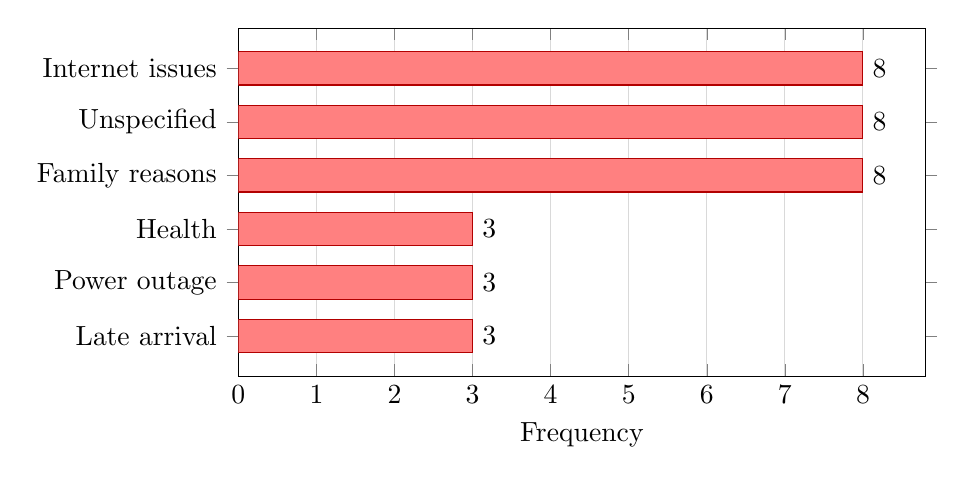
\begin{tikzpicture}
\begin{axis}[
    width=0.85\textwidth,
    height=6cm,
    xbar,
    xlabel={Frequency},
    symbolic y coords={{Late arrival}, {Power outage}, {Health}, {Family reasons}, {Unspecified}, {Internet issues}},
    ytick=data,
    nodes near coords,
    nodes near coords align={horizontal},
    bar width=12pt,
    xmin=0,
    enlarge y limits=0.15,
    xmajorgrids=true,
    ymajorgrids=false,
    grid style={gray!30},
]
\addplot[fill=red!50, draw=red!70!black] coordinates {(3,{Late arrival}) (3,{Power outage}) (3,{Health}) (8,{Family reasons}) (8,{Unspecified}) (8,{Internet issues})};
\end{axis}
\end{tikzpicture}
\caption{Distribution of absence reasons reflecting wartime education conditions}
\label{fig:absence}
\end{figure}

\subsection{Wartime context}

The absence data provide a vivid picture of education under wartime conditions \cite{UNESCO2023, Humeniuk2022113}. Three categories of absences are directly attributable to the conflict:

\textbf{Infrastructure disruptions (33.3\%).} Internet problems (24.2\%) and power outages (9.1\%) together account for one-third of all reported absences. These are characteristic of wartime conditions in Kryvyi Rih, where missile and drone attacks frequently damage energy infrastructure, causing both immediate blackouts and cascading internet disruptions.

Representative messages from the chat log illustrate these challenges:
\begin{itemize}
\item ``добрий день. в мене зникло світло, буду відсутня на занятті'' (Dec 1, 2024, Булахова Наталя)
\item ``У мене поганий інтернет'' (Dec 29, 2024, Саша Зоріна)
\item ``Інтернету немає'' (Apr 13, 2025, Віолетта)
\item ``Інтернет в мене накрився остаточно'' (Dec 8, 2024, instructor)
\end{itemize}

Notably, the instructor himself experienced internet disruptions (December 8, 2024; February 16, 2025), demonstrating that wartime conditions affect all participants. The course adapted by providing asynchronous alternatives: all lecture recordings, presentation files, and quiz links were shared through the chat group and Google Drive, reflecting the principles of emergency remote teaching \cite{Striuk_2022, Hlianenko2024}.

The instructor explicitly addressed safety concerns on February 2, 2025:
\begin{quote}
``Ваша безпека найважливіша [...] Я не в місті, тому продовжую заняття, і Ви можете лишатися якщо почуваєтеся в безпеці, якщо є сумніви -- краще перейдіть в укриття. Записи лекцій публікуються тут після кожного заняття.'' (Your safety is the most important [...] I am not in the city, so I continue the classes, and you can stay if you feel safe; if in doubt, go to a shelter. Lecture recordings are published here after each session.)
\end{quote}

This message exemplifies the pedagogical adaptation required in wartime: prioritising student safety while maintaining educational continuity through asynchronous materials \cite{UNESCO2023}.

\textbf{Temporal distribution of absences.} Table~\ref{tab:absence-temporal} presents the temporal distribution of absence reports across the six-month course period. Absences were not evenly distributed: the months with the highest absence frequency were April 2025 (8 reports), February 2025 (7 reports), and December 2024 (6 reports). The peak in December and the April increase coincide with periods of intensified military activity affecting Kryvyi Rih's energy infrastructure \cite{Humeniuk2022113}, while February absences were more often attributed to family circumstances.

\begin{table}[htbp]
\centering
\caption{Temporal distribution of absence reports by month and reason category}
\label{tab:absence-temporal}
\small
\begin{tabular}{lccccccc}
\hline
\textbf{Month} & \textbf{Infra.} & \textbf{Family} & \textbf{Health} & \textbf{Unspec.} & \textbf{Late} & \textbf{Total} \\
\hline
October 2024  & 1 & 0 & 0 & 0 & 0 & 1 \\
November 2024 & 1 & 0 & 0 & 0 & 0 & 1 \\
December 2024 & 4 & 0 & 1 & 1 & 0 & 6 \\
January 2025  & 1 & 0 & 0 & 1 & 0 & 2 \\
February 2025 & 0 & 3 & 1 & 2 & 1 & 7 \\
March 2025    & 0 & 3 & 0 & 1 & 0 & 4 \\
April 2025    & 4 & 1 & 0 & 1 & 2 & 8 \\
\hline
\textbf{Total} & \textbf{11} & \textbf{7} & \textbf{2} & \textbf{6} & \textbf{3} & \textbf{29} \\
\hline
\end{tabular}
\end{table}

\textit{Note:} The totals in Table~\ref{tab:absence-temporal} differ slightly from Table~\ref{tab:absence-reasons} because some messages contained multiple absence indicators classified separately, and CDPO administrative messages about attendance are excluded from temporal analysis.

\textbf{Individual absences by student.} Analysis of individual absence patterns reveals that absences were concentrated among a subset of students (Table~\ref{tab:individual-absence}).

\begin{table}[htbp]
\centering
\caption{Individual absence frequency and primary reasons}
\label{tab:individual-absence}
\small
\begin{tabular}{lcl}
\hline
\textbf{Student} & \textbf{Absences} & \textbf{Primary reasons} \\
\hline
Sasha Zorina & 7 & Internet (3), Family (2), Unspecified (2) \\
Yana & 5 & Internet (1), Family (1), Power (1), Unspecified (2) \\
Bulakhova N. & 5 & Power (2), Internet (1), Unspecified (2) \\
Violetta & 3 & Internet (1), Late (1), Unspecified (1) \\
Nastya & 2 & Family (1), Internet (1) \\
Khaitmatova A. & 2 & Family (1), Late (1) \\
Other (5 students) & 5 & 1 each \\
\hline
\end{tabular}
\end{table}

The concentration of absences among three students (Sasha Zorina, Yana, and Bulakhova N.) is noteworthy. These three students account for 17 of 33 absence reports (51.5\%). Despite their frequent absences from synchronous sessions, all three remained enrolled throughout the course, suggesting that the asynchronous materials (recorded lectures, shared quiz links, Google Drive resources) enabled continued participation -- a finding that supports the resilience value of multi-channel distance education delivery \cite{Tamim2011, UNESCO2023}. Bulakhova N.'s absences were predominantly infrastructure-related (power outages and internet problems), making her case a particularly clear example of wartime impact on educational access.

\textbf{Cross-referencing absences with performance.} Comparing the absence data with the individual trajectory data (Table~\ref{tab:trajectories}) reveals an interesting pattern. Violetta, who reported 3 absences, still appeared in 5 seminar datasets with a mean score of 47.0\%, suggesting that despite synchronous session interruptions, she maintained assessment engagement. Conversely, Sasha Zorina, with the highest absence count (7), did not appear in any of the analysed response datasets (Seminars 25--39), indicating that her absences extended beyond synchronous sessions to assessment participation.

The concentration of absences among a subset of students, combined with their continued enrollment and quiz participation, suggests that these students maintained engagement with the course through asynchronous materials despite being unable to attend synchronous sessions regularly. This finding aligns with research on the role of digital technologies in maintaining educational continuity during crises \cite{UNESCO2023, Striuk_2022}.

\subsection{Course timeline overview}

Figure~\ref{fig:timeline} presents a comprehensive timeline of all assessment activities throughout the course, distinguishing between seminar quizzes, modular controls, lecture quizzes, and the introductory test.

\begin{figure}[htbp]
\centering
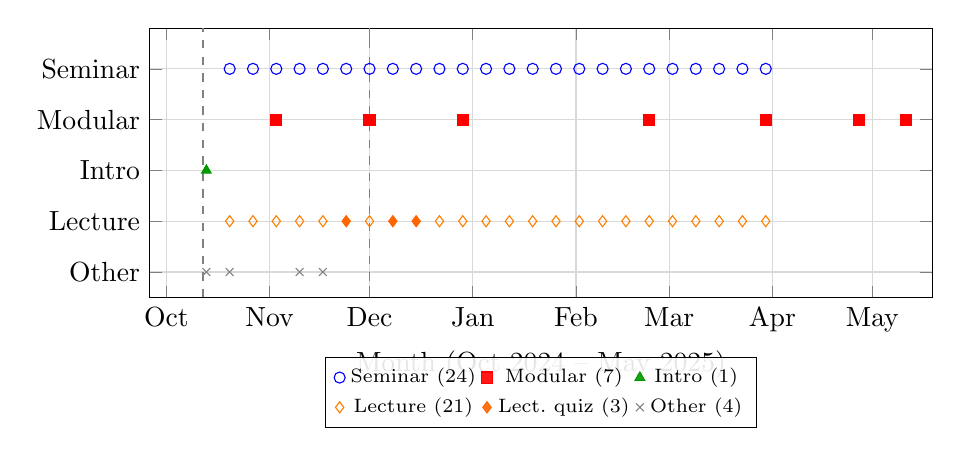
\begin{tikzpicture}
\begin{axis}[
    width=0.95\textwidth,
    height=5cm,
    xlabel={Month (Oct 2024 -- May 2025)},
    xticklabels={Oct, Nov, Dec, Jan, Feb, Mar, Apr, May},
    xtick={0,31,61,92,123,151,182,212},
    yticklabels={Other, Lecture, Intro, Modular, Seminar},
    ytick={0,1,2,3,4},
    grid=major,
    grid style={gray!30},
    legend style={at={(0.5,-0.22)}, anchor=north, font=\scriptsize, legend columns=3, fill=white, fill opacity=0.9, draw opacity=1, text opacity=1},
    ymin=-0.5, ymax=4.8,
    xmin=-5, xmax=230,
]
\addplot[only marks, mark=o, mark size=2pt, blue] coordinates {(19,4) (26,4) (33,4) (40,4) (47,4) (54,4) (61,4) (68,4) (75,4) (82,4) (89,4) (96,4) (103,4) (110,4) (117,4) (124,4) (131,4) (138,4) (145,4) (152,4) (159,4) (166,4) (173,4) (180,4)};
\addlegendentry{Seminar (24)}
\addplot[only marks, mark=square*, mark size=2pt, red] coordinates {(33,3) (61,3) (89,3) (145,3) (180,3) (208,3) (222,3)};
\addlegendentry{Modular (7)}
\addplot[only marks, mark=triangle*, mark size=2pt, green!60!black] coordinates {(12,2)};
\addlegendentry{Intro (1)}
\addplot[only marks, mark=diamond, mark size=2pt, orange] coordinates {(19,1) (26,1) (33,1) (40,1) (47,1) (61,1) (82,1) (89,1) (96,1) (103,1) (110,1) (117,1) (124,1) (131,1) (138,1) (145,1) (152,1) (159,1) (166,1) (173,1) (180,1)};
\addlegendentry{Lecture (21)}
\addplot[only marks, mark=diamond*, mark size=2pt, orange!80!red] coordinates {(54,1) (68,1) (75,1)};
\addlegendentry{Lect.\ quiz (3)}
\addplot[only marks, mark=x, mark size=2pt, gray] coordinates {(12,0) (19,0) (40,0) (47,0)};
\addlegendentry{Other (4)}
\draw[dashed, gray] (axis cs:11,-0.5) -- (axis cs:11,4.8) node[above, font=\tiny, text=gray] {Start};
\draw[dashed, gray] (axis cs:61,-0.5) -- (axis cs:61,4.8) node[above, font=\tiny, text=gray] {Gamification};
\end{axis}
\end{tikzpicture}

\caption{Complete course assessment timeline (October 2024 -- April 2025)}
\label{fig:timeline}
\end{figure}

The timeline reveals several important patterns:
\begin{itemize}
\item Assessment frequency was relatively consistent throughout the course, with seminars held approximately weekly;
\item Modular controls were evenly distributed across the six-month period;
\item There was a brief reduction in activity around late December 2024 -- early January 2025 (winter holidays), followed by intensified activity;
\item The gamification platform \cite{Korniienko2025els, Titova2025cte} was introduced at the midpoint of the course (December 1, 2024), providing supplementary assessment and practice opportunities for the second half.
\end{itemize}


\section{Discussion} \label{sec:discussion}

\subsection{Interpretation of findings in context of the systematic reviews}

The findings of this experimental study should be interpreted in light of the theoretical framework established in Chapter~\ref{ch:theory} and the systematic reviews of gamification in history education \cite{KorniienkoSemerikov2024, Korniienko2025els}:

\textbf{Addressing the research quality gap.} One of the central findings of the MRQS assessment \cite{Korniienko2025mrqs} (Section~\ref{sec:mrqs}) was that 83.8\% of gamification studies in history education carried a high risk of bias, primarily due to lack of transparency in reporting. This finding echoes broader concerns about research quality in educational technology \cite{Clark2016, Connolly2012} and gamification research specifically \cite{DichevDicheva2017, KoivistoHamari2019}. This study addresses several of the identified weaknesses:

\begin{itemize}
\item \textbf{Complete documentation}: The chat log, response data, gamification platform source code, and analysis pipeline are all preserved and can be made available for verification and replication.
\item \textbf{Transparent limitations}: The limitations of the data and design are explicitly acknowledged, including the small sample size, rolling enrollment, and absence of a control group.
\item \textbf{Operational definitions}: Gamification is clearly defined as the integration of game design elements (creative quiz naming, interactive web-based exercises, immediate feedback, progressive difficulty) into the non-game context of NMT history preparation, following the canonical definition by \citet{Deterding2011}.
\end{itemize}

\subsection{Pre-gamification vs post-gamification comparison}

The availability of response data for 36 seminars spanning both the pre-gamification (Seminars 1--24, N=23) and post-gamification (Seminars 25--39, N=13) periods enables a descriptive comparison of the two phases. Figure~\ref{fig:pre-post} summarises the key differences.

\begin{figure}[htbp]
\centering
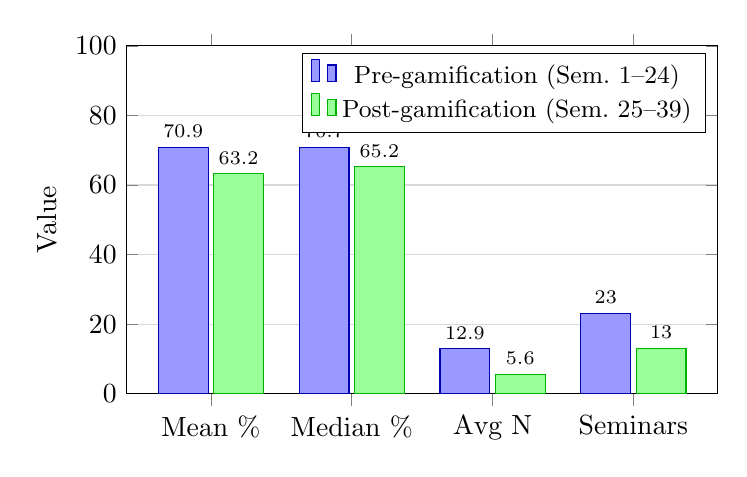
\begin{tikzpicture}
\begin{axis}[
    width=0.75\textwidth,
    height=6cm,
    ybar,
    bar width=18pt,
    ylabel={Value},
    symbolic x coords={Mean \%, Median \%, Avg N, Seminars},
    xtick=data,
    ymin=0, ymax=100,
    legend style={at={(0.98,0.98)}, anchor=north east, font=\small},
    nodes near coords,
    nodes near coords style={font=\scriptsize},
    enlarge x limits=0.2,
    xmajorgrids=false,
    ymajorgrids=true,
    grid style={gray!30},
]
\addplot[fill=blue!40, draw=blue!70!black] coordinates {
    ({Mean \%},70.9)
    ({Median \%},70.7)
    ({Avg N},12.9)
    ({Seminars},23)
};
\addlegendentry{Pre-gamification (Sem.\ 1--24)}

\addplot[fill=green!40, draw=green!70!black] coordinates {
    ({Mean \%},63.2)
    ({Median \%},65.2)
    ({Avg N},5.6)
    ({Seminars},13)
};
\addlegendentry{Post-gamification (Sem.\ 25--39)}
\end{axis}
\end{tikzpicture}
\caption{Summary comparison of pre-gamification (Seminars 1--24) and post-gamification (Seminars 25--39) periods}
\label{fig:pre-post}
\end{figure}

The pre-gamification period shows a higher overall mean score (70.7\% vs 63.4\%) and higher average participation (N=12.7 vs N=5.6). However, this comparison must be interpreted with several important caveats:

\begin{itemize}
\item \textbf{Topic difficulty confound}: The pre-gamification seminars covered earlier historical periods (ancient through early modern Ukraine), while the post-gamification seminars covered more complex modern and contemporary periods, including comprehensive NMT-format assessments. Topic difficulty is a known confound in longitudinal educational studies \cite{Clark2016, Connolly2012}.
\item \textbf{Assessment format differences}: Many post-gamification seminars used comprehensive, multi-period assessment formats (e.g., Seminar 37 based on the 2016 NMT), while pre-gamification seminars focused on specific historical periods.
\item \textbf{Participation decline}: The declining N in post-gamification seminars partly reflects the voluntary nature of quiz completion and the wartime attrition documented in Section~\ref{sec:attendance}.
\item \textbf{Rolling enrollment}: Students who joined later in the course had less preparation time, potentially lowering post-gamification group averages.
\end{itemize}

These confounds preclude causal attribution of score differences to the gamification intervention. The single-group design without random assignment means that any observed differences may reflect topic difficulty, assessment format, participant characteristics, or other unmeasured variables \cite{creswell, Korniienko2025mrqs}. Nevertheless, the data provide a comprehensive descriptive baseline for the complete course trajectory.

\textbf{Consistency with the effectiveness literature.} The predominantly positive engagement patterns observed (continued participation, quiz completion, chat interactions) are consistent with the 70.3\% of studies in the systematic review \cite{Korniienko2025els} that reported positive effects on engagement. This aligns with the meta-analytic findings of \citet{Hamari2014}, who reported generally positive effects of gamification on engagement across educational contexts, and with the reviews by \citet{KoivistoHamari2019} and \citet{Sailer2017}. However, the variable score results (33.3\%--83.3\% across seminars) reflect the reality that engagement does not automatically translate to academic achievement \cite{Clark2016, Connolly2012} -- a nuance that the 10.8\% of studies reporting negative or mixed results also captured \cite{KorniienkoSemerikov2024}.

\textbf{Design principles in practice.} The six design principles identified in the systematic review \cite{Korniienko2025els, KorniienkoSemerikov2024} were implemented in this study, drawing on evidence from both the gamification literature \cite{Sailer2017, Qian2016} and digital history pedagogy \cite{Korniienko2025cte}. Table~\ref{tab:design-principles-impl} maps each principle to specific implementation elements and the evidence of their application.

\begin{table}[htbp]
\centering
\caption{Implementation of evidence-based design principles}
\label{tab:design-principles-impl}
\small
\begin{tabular}{p{3cm}p{4.5cm}p{5cm}}
\hline
\textbf{Principle} & \textbf{Implementation} & \textbf{Evidence} \\
\hline
Historical authenticity & All quiz content aligned with the NMT curriculum and verified historical facts & 156 Google Forms with NMT-format questions; 38 lectures covering the complete Ukrainian history curriculum \\
\hline
Narrative integration & Creative thematic naming for quiz blocks (Greek mythology, gemstones, flowers, trees, minerals) & Chat log records naming schemes for Seminars 17--30; students acknowledged naming in chat \\
\hline
Progressive difficulty & Chronological progression from ancient to modern history; comprehensive tests at intervals & Course structure from Section 1 (Ancient/Medieval) through Section 4 (20th century) to Omega (comprehensive) \\
\hline
Immediate feedback & Google Forms auto-scoring; HistoryLikeGame colour-coded feedback & Score display in ``X/Y'' format after submission; green/red visual feedback in game modules \\
\hline
Social elements & Viber group interactions; collaborative encouragement; CDPO attendance messages & 400 chat messages; instructor support messages; peer interaction \\
\hline
Multiple modalities & Quizzes, videos, presentations, worksheets, interactive drag-and-drop games, text input exercises & 38 lecture recordings, 30+ worksheets, 23 game modules, 156 quiz forms \\
\hline
\end{tabular}
\end{table}

The implementation of all six principles simultaneously distinguishes this study from the majority of gamification implementations reviewed in Section~\ref{sec:gamification-review} \cite{KorniienkoSemerikov2024, Korniienko2025els}, where studies typically employed only 1--3 principles. For example, \citet{1Barbatsis201159} focused primarily on narrative integration, while \citet{16Chen201447} emphasised social elements, and \citet{55Squire2004} combined historical authenticity with narrative integration. The comprehensive approach in the present study reflects the implementation guidelines developed in Section~\ref{sec:digcomp} \cite{Titova2025cte, Titova_Korniienko} and aligned with DigComp~2.0 \cite{Vuorikari2016}.

\textbf{Score patterns and question difficulty.} The wide variation in mean scores across seminars (33.3\%--83.3\%) warrants interpretation in relation to the effectiveness literature. The systematic review \cite{Korniienko2025els} found that 51.4\% of studies reported positive effects on learning outcomes, consistent with the broader meta-analyses by \citet{Clark2016} and \citet{Connolly2012}. In this study, the pattern is more nuanced: high scores on period-specific assessments (Seminars 25, 31, 32, 35: mean 77.1\%--83.3\%) and lower scores on comprehensive NMT-format assessments (Seminars 36, 37: mean 50.7\%--59.6\%) suggest that the gamification-enhanced course was effective for topic-specific learning but that comprehensive integration of knowledge across historical periods remained challenging. This aligns with the 37.8\% of studies in the review that found no significant difference in broader achievement measures \cite{KorniienkoSemerikov2024}. Similar patterns of differential effectiveness across assessment types have been reported by \citet{8Yu2014} and \citet{6Czerwinski2018} in their respective gamification implementations in history education.

\textbf{The repeated-attempt phenomenon.} The case of Talash D. (Section~\ref{sec:formative}), who submitted 7 attempts at Seminar 37 with progressively improving scores, illustrates a mechanism not frequently discussed in the gamification literature \cite{DichevDicheva2017}: the use of immediate feedback to drive iterative mastery. This behaviour pattern, enabled by the design principle of immediate feedback \cite{Sailer2017}, resembles the ``mastery learning'' approach described by \citet{Hattie2009}, where students are given multiple opportunities to achieve competence. The fact that Talash D.'s subsequent score on Seminar 39 (82.8\%) was substantially higher than his first attempt on Seminar 37 (18.9\%) provides tentative evidence for the lasting value of this iterative approach. Among the reviewed studies, similar repeated-attempt mechanisms were observed in web-based game implementations such as \citet{5kazanidis2018alpha} and \citet{50Lye2013}, though neither study examined the phenomenon in the depth enabled by the present study's multi-assessment design.

\subsection{Wartime education implications}

The study provides unique documentation of distance history education under active conflict conditions \cite{UNESCO2023}. Several findings have broader implications for educational policy and practice in conflict-affected settings, contributing to the limited empirical literature on education in conflict zones \cite{Humeniuk2022113, Striuk_2022}.

\textbf{Resilience through redundancy.} The multi-channel approach (Zoom for synchronous sessions, Viber for communication, Google Drive for materials, Google Forms for assessment, HistoryLikeGame for supplementary practice) ensured that disruption of any single channel did not prevent learning \cite{Tamim2011}. This redundancy was tested repeatedly during the course:

\begin{itemize}
\item When the instructor lost internet on December 8, 2024, recorded lectures had already been shared through the Viber group and Google Drive, allowing students to access the material asynchronously.
\item When students experienced power outages (e.g., Bulakhova N. on December 1, 2024; Yana on December 15, 2024), quiz links remained available in the chat history for later completion.
\item During the April 13, 2025 session, multiple students reported simultaneous internet problems (Bulakhova N., Violetta, Nastya), suggesting a regional infrastructure disruption. The pre-shared materials and asynchronous quiz availability ensured that learning continued.
\end{itemize}

The resilience model can be conceptualised as a five-layer architecture:

\begin{enumerate}
\item \textbf{Synchronous layer} (Zoom): Primary instruction; most vulnerable to disruptions.
\item \textbf{Communication layer} (Viber): Asynchronous messaging; low bandwidth requirements.
\item \textbf{Content layer} (Google Drive): Stored materials; accessible when internet is available.
\item \textbf{Assessment layer} (Google Forms): Asynchronous completion possible; data preserved.
\item \textbf{Gamification layer} (HistoryLikeGame): Static HTML; minimal bandwidth; offline-capable once loaded.
\end{enumerate}

Each layer provides a fallback when higher layers fail. This architecture was not planned as a wartime resilience strategy but emerged organically from the multi-tool approach to distance education \cite{Striuk_2022, UNESCO2023}, demonstrating that pedagogical diversity can serve as an unintentional resilience mechanism. The layered approach aligns with the technology integration frameworks discussed in the educational technology literature \cite{Ertmer1999, Davis2017, Middleton2014192}.

\textbf{Infrastructure as a research variable.} In wartime contexts, infrastructure reliability becomes a research variable rather than an assumed constant \cite{UNESCO2023}. The 33.3\% of absences attributable to infrastructure failures (internet + power) demonstrates the need for educational research frameworks that account for environmental instability. Standard research quality criteria \cite{Korniienko2025mrqs, HigginsThomas2019} (e.g., attendance rates, completion rates, assessment timing) must be reinterpreted when participants face physical dangers and infrastructure disruptions beyond their control.

The temporal analysis of infrastructure-related absences (Table~\ref{tab:absence-temporal}) reveals that these disruptions were not uniformly distributed but clustered in specific months (December 2024 and April 2025), corresponding to periods of intensified military activity. This clustering suggests that infrastructure disruptions are not random noise but systematic factors that covary with external military events, a finding with implications for research design in conflict-affected education contexts \cite{UNESCO2023, Humeniuk2022113}.

\textbf{Gamification's accessibility advantage.} The HistoryLikeGame platform's design as static HTML pages with minimal bandwidth requirements was validated by the wartime context. Unlike VR/AR implementations that dominate the gamification literature \cite{KorniienkoSemerikov2024, 13Humpire2022, 15Slater2022} or streaming video and complex web applications, the gamified exercises remained accessible even under degraded network conditions. The platform's total size (approximately 200~KB for all 23 modules, based on the catalogue data in Table~\ref{tab:game-modules}) is significantly smaller than a single lecture recording or presentation file, making it the most accessible component of the course infrastructure. This lightweight approach contrasts with the technology-intensive implementations reported by \citet{31DeAmicis2009451} and \citet{14Forsyth2023}, and demonstrates that effective gamification does not require sophisticated technology \cite{Deterding2011, Peixoto2015}.

\textbf{Safety prioritisation in pedagogy.} The instructor's February 2, 2025 message about prioritising safety over attendance represents an important pedagogical stance in conflict settings \cite{UNESCO2023}. By explicitly stating that ``your safety is the most important'' and providing asynchronous alternatives, the course established a norm where physical safety was never compromised for educational continuity. This approach differs from the pre-war expectation of mandatory synchronous attendance \cite{MON} and represents an adaptation that other conflict-affected educational programmes may need to adopt.

\textbf{The role of community in wartime education.} The Viber chat group served not only as a communication channel but as a support community. Students' absence messages, while documenting disruptions, also demonstrated a sense of obligation to the group -- they informed the instructor and peers rather than simply not appearing. This social element, identified as one of the six design principles of gamification \cite{Korniienko2025els, Sailer2017}, took on additional significance in the wartime context where shared challenges can either fragment or strengthen community bonds \cite{UNESCO2023}. The social dynamics observed here resonate with research on collaborative learning and social presence in online environments \cite{Bonwell1991, Prensky2001, Syn2020909}.

\subsection{Limitations}

The following limitations should be considered when interpreting the results:

\begin{enumerate}
\item \textbf{Data coverage}: Response data are available for 36 of 30 planned seminars (Seminars 1--39, excluding 8 and 38) and all 7 modular controls, covering the full pre-gamification and post-gamification periods. While this represents substantial coverage, the pre-gamification data were recovered from multi-sheet XLSX files with aggregated per-student averages, limiting the granularity of individual-level analysis in that period. Direct before-after comparison is further complicated by confounding variables (topic difficulty, assessment format, enrollment changes) \cite{DichevDicheva2017, Korniienko2025mrqs}.

\item \textbf{Small and variable sample sizes}: The number of respondents per seminar (1--15) limits the power of statistical analyses and the generalisability of findings \cite{Cohen2005, Borenstein2009}. In particular, Seminars 28 and 30 had only 1 respondent each, making their scores essentially individual case data rather than group statistics.

\item \textbf{Absence of control group}: The single-group design precludes causal attribution of outcomes to the gamification intervention \cite{Schulz2010CONSORT, creswell}. The ethical and practical impossibility of withholding educational resources from enrolled students meant that a traditional experimental design was not feasible in this context, a common constraint in educational gamification research \cite{Korniienko2025mrqs, Reeves2003}.

\item \textbf{Self-selection bias}: Students who completed quizzes may differ systematically from those who did not, potentially inflating apparent performance \cite{ary, creswell}. The analysis of named participants (Table~\ref{tab:trajectories}) shows that high-performing students tended to participate in more seminars, which is consistent with self-selection.

\item \textbf{Rolling enrollment}: The continuous influx of new students (23 unique joins across three distinct phases) makes it difficult to track cohort-level progression. Students who enrolled in April 2025 had access to only the final weeks of the course, while those enrolled from October 2024 had the full six months.

\item \textbf{Limited demographic data}: Participants' characteristics beyond names are not available. Variables such as prior academic performance, motivation level, access to technology, geographic location within Ukraine, and proximity to conflict zones -- all potentially confounding factors -- were not collected. The importance of such demographic variables in gamification research has been emphasised by \citet{KoivistoHamari2019} and \citet{Hamari2014}.

\item \textbf{Name inconsistency}: Some students used different name formats across quiz forms (e.g., ``Каменєва Анастасія'' and ``Каменєва Настя''; ``Софія Вовк'' and ``Вовк Софія''), complicating individual trajectory tracking. While these were resolved through manual matching, some responses may remain unlinked.

\item \textbf{Gamification platform usage data}: The HistoryLikeGame platform, being composed of static HTML files, does not track user interactions or completion rates. Usage data are therefore limited to the chat log mentions of the platform, preventing a direct assessment of platform engagement.
\end{enumerate}

These limitations are consistent with the constraints identified in the MRQS review \cite{Korniienko2025mrqs} (Section~\ref{sec:mrqs}) and are reported here in accordance with the recommendations for improved transparency in educational research \cite{Page2021, Moher2009PRISMA}. Notably, several of these limitations (small sample, no control group, rolling enrollment) are characteristic of the 83.8\% of gamification studies assessed as high risk of bias \cite{Korniienko2025mrqs}. The critical difference is that this study explicitly acknowledges and documents these limitations rather than presenting results without qualification, following best practices in reporting standards \cite{Schulz2010CONSORT, Page2021}.

\subsection{Comparison with MRQS quality criteria}

Following the self-assessment approach recommended in the MRQS framework \cite{Korniienko2025mrqs}, this study can be evaluated against the five quality domains, adapting quality assessment tools from the broader systematic review methodology \cite{HigginsThomas2019, Wells2014, Whiting2016}. Table~\ref{tab:self-assessment} presents the domain-by-domain assessment with detailed justifications.

\begin{table}[htbp]
\centering
\caption{Self-assessment of the current study against MRQS criteria}
\label{tab:self-assessment}
\small
\begin{tabular}{llp{7cm}}
\hline
\textbf{Domain} & \textbf{Rating} & \textbf{Justification} \\
\hline
Research design & Moderate risk & Ex post facto design appropriate for the context; lacks randomisation and control group; design chosen for ecological validity rather than internal validity \\
\hline
Sampling & Moderate risk & Complete cohort studied (N=23); no power analysis; sample size below the 50-participant threshold identified as minimum in the MRQS review \\
\hline
Data collection & Low risk & Established instruments (Google Forms with automatic scoring); systematic data pipeline with reproducible code; multiple data sources (quiz responses, chat log, platform analysis) \\
\hline
Data analysis & Low risk & Appropriate descriptive methods for sample sizes; limitations acknowledged; automated pipeline ensures reproducibility; no inappropriate inferential statistics applied to small samples \\
\hline
Reporting & Low risk & Comprehensive documentation of methods, materials, and analysis code; transparent limitation reporting; operational definitions provided; raw data preservation \\
\hline
\textbf{Overall} & \textbf{Moderate} & Three domains at low risk; two at moderate risk. Overall rating: moderate risk, placing this study in the top 16.2\% of reviewed studies \\
\hline
\end{tabular}
\end{table}

This self-assessment places the current study in the moderate risk category -- above the 83.8\% of studies assessed as high risk in the systematic review \cite{Korniienko2025mrqs}. The study's primary strengths lie in the data collection, data analysis, and reporting domains, where comprehensive documentation, systematic pipeline processing, and transparent limitation reporting address the most common weaknesses identified in the reviewed literature \cite{KorniienkoSemerikov2024}. The acknowledged limitations in research design and sampling are inherent to the educational context \cite{Reeves2003} and represent honest constraints rather than methodological oversights.

The MRQS self-assessment also reveals an important meta-methodological finding: by conducting and publishing the quality assessment alongside the study results, researchers can demonstrate awareness of their study's position within the field's quality spectrum \cite{Korniienko2025mrqs, GuyattGRADE2008}. This practice, if adopted widely, could contribute to the gradual improvement of research quality in gamification education research that the MRQS review identified as urgently needed \cite{KorniienkoSemerikov2024, Korniienko2025els}.

\subsection{Comparison with the gamification evidence base}

The findings of this study can be contextualised against the 74-study evidence base reviewed in Chapter~\ref{ch:theory} \cite{KorniienkoSemerikov2024, Korniienko2025els}. Several points of comparison merit discussion.

\textbf{Course duration.} This study's six-month duration (October 2024 -- April 2025) places it among the longest gamification implementations documented in the reviewed literature \cite{Korniienko2025els}. Among the 17 studies that reported specific intervention durations, the range was extremely broad -- from 7 minutes \cite{1Barbatsis201159} to 30 hours, with 8 studies involving interventions of 20 minutes or less \cite{11Ternblad2023115, 21Ghulamani2017}. Only four studies involved extended implementations exceeding one week \cite{55Squire2004, 46Stirling2022, 9Lin2018, 48Moketar2021}. The extended duration of the present study provides an opportunity to examine long-term engagement patterns and score trajectories that brief interventions cannot capture, addressing a gap identified by \citet{KoivistoHamari2019} and \citet{Hernandez2017}.

\textbf{Assessment volume.} The 156 Google Forms quizzes administered during the course represent a substantially larger assessment dataset than most reviewed studies \cite{KorniienkoSemerikov2024}. This volume enables the identification of performance patterns across historical periods and the tracking of individual learning trajectories -- analyses that were not possible in the many studies that relied on single pre-post test comparisons \cite{16Chen201447, 6Czerwinski2018, 8Yu2014}.

\textbf{Game type classification.} Within the taxonomy developed in the systematic review \cite{Korniienko2025els}, the HistoryLikeGame platform is best classified as a ``web-based game'' (13.5\% of the review corpus), alongside implementations by \citet{5kazanidis2018alpha}, \citet{50Lye2013}, and \citet{43ali2018indonesian}, while the broader course gamification (creative quiz naming, thematic structures, multiple platforms) incorporates elements of ``structural gamification'' (adding game elements to existing content) \cite{Deterding2011}. The platform's HTML-based architecture distinguishes it from the VR/AR implementations that dominate the field (25.7\%) \cite{13Humpire2022, 15Slater2022, 10Huaman2019220} by prioritising accessibility and resilience over immersion.

\textbf{Outcome patterns.} The review found that 70.3\% of studies reported positive effects on engagement \cite{Korniienko2025els, KorniienkoSemerikov2024}. The present study's evidence for engagement is indirect but suggestive: the increase in participation from early seminars (N = 1--3) to later ones (N = 12--15), the high frequency of participation among core students (e.g., Svintsitska V. appearing in 9 of 13 seminars), and the repeated-attempt behaviour of Talash D. all suggest positive engagement effects, consistent with the findings of \citet{Hamari2014} and \citet{Sailer2017}. The learning outcome pattern (high scores on topic-specific assessments, lower scores on comprehensive assessments) aligns with the review's finding that effect sizes were stronger for factual recall than for interpretive understanding \cite{Clark2016, Connolly2012}. Similar differential effects have been reported in history-specific implementations by \citet{53Perez2014}, \citet{54Gibson2007}, and \citet{59Kee2014270}.

\textbf{Gamification definition.} This study contributes to addressing the definitional ambiguity identified in 85.1\% of reviewed studies \cite{Korniienko2025els} by explicitly categorising the course as employing a combination of structural gamification (creative quiz naming, point-based scoring, progression through sections), content gamification (thematic quiz blocks, narrative integration through historical period structure), and a game-based learning component (the HistoryLikeGame platform), following the definitional framework of \citet{Deterding2011}. This multi-category approach demonstrates that real-world implementations often blend the four conceptual approaches identified in the review \cite{KorniienkoSemerikov2024} rather than employing a single pure approach, a finding also noted in broader gamification reviews \cite{SEABORN201514, Zhonggen2019, Unkelos-Shpigel2016}.

\subsection{Implications for digital history methodology}

This study contributes to the broader thesis argument that digital history methodology encompasses a range of digital tools and approaches \cite{Korniienko2025cte, Crymble2021}, of which gamification is one component \cite{Deterding2011}. The PRISMA review of digital history pedagogy \cite{Korniienko2025cte} (Section~\ref{sec:dh-review}) identified only 6 studies, while the gamification review \cite{Korniienko2025els} identified 74 -- a 12-fold difference that underscores gamification's prominence within the digital history landscape.

The present study demonstrates that digital history methodology in practice is not limited to any single digital tool \cite{CohenRosenzweig2006} but involves the integration of multiple digital platforms and approaches:

\begin{itemize}
\item \textbf{Digital communication} (Viber for synchronous and asynchronous messaging);
\item \textbf{Digital content delivery} (Zoom for video lectures, Google Drive for materials);
\item \textbf{Digital assessment} (Google Forms for quiz-based formative assessment);
\item \textbf{Digital gamification} (HistoryLikeGame for interactive practice, Wordwall for variety);
\item \textbf{Digital archiving} (recorded lectures, preserved chat logs, response data).
\end{itemize}

This integration of digital tools addresses all five DigComp 2.0 competence areas \cite{Vuorikari2016} (Section~\ref{sec:digcomp}) and provides a practical model for comprehensive digital history methodology \cite{Titova2025cte, Titova_Korniienko}. The methodology goes beyond the ``technology-as-supplement'' approach that characterised many reviewed studies \cite{Korniienko2025els, KorniienkoSemerikov2024} and approaches the ``technology-as-infrastructure'' paradigm \cite{Ertmer1999} where digital tools become the medium through which education is delivered, assessed, and documented. This paradigm aligns with the comprehensive digital competence development framework proposed by \citet{Humeniuk2022113} and \citet{Nunez202329} and the software engineering education gamification approaches reviewed by \citet{Korniienko2025aredu}.

\subsection{Future research directions}

Based on the findings and limitations of this study, several directions for future research can be identified:

\begin{enumerate}
\item \textbf{Controlled comparison studies}: Future implementations should include control groups (e.g., parallel sections of the same course with and without gamification) to enable causal inference about gamification effectiveness \cite{Schulz2010CONSORT, creswell}. The MRQS review \cite{Korniienko2025mrqs} found that control group usage declined over time ($-$13.5 percentage points), making this an increasingly urgent need. Experimental designs such as those employed by \citet{16Chen201447} and \citet{6Czerwinski2018} could serve as models.

\item \textbf{Platform analytics}: Future versions of HistoryLikeGame should incorporate usage tracking (module completion times, attempt counts, interaction patterns) to provide direct evidence of gamification engagement \cite{Sailer2017, KoivistoHamari2019} rather than relying on indirect indicators from quiz scores and chat logs.

\item \textbf{Larger samples}: Scaling the approach to multiple CDPO course sections or multiple institutions would address the sample size limitation \cite{Cohen2005, Borenstein2009} and enable subgroup analyses (e.g., by enrollment phase, by geographic region, by prior academic performance), following the recommendations of \citet{Korniienko2025mrqs}.

\item \textbf{Longitudinal follow-up}: Tracking participants' NMT scores after course completion would provide a direct outcome measure for the effectiveness of the gamification-enhanced preparation programme.

\item \textbf{Student perspectives}: Incorporating structured interviews or surveys would capture qualitative data on student perceptions of the gamification elements \cite{Hamari2014, DichevDicheva2017}, their preferred learning modalities, and their experience of learning under wartime conditions \cite{UNESCO2023, Ditlmann2025}.

\item \textbf{Comparative domain analysis}: Extending the approach to other NMT subjects (Mathematics, Ukrainian Language and Literature) would test the generalisability of the gamification methodology beyond history education. The SE education review \cite{Korniienko2025aredu} demonstrated that gamification approaches in software engineering education share common design principles with those in history education, suggesting cross-domain applicability.

\item \textbf{Replication across conflict contexts}: The wartime education findings have potential relevance for other conflict-affected educational settings worldwide \cite{UNESCO2023}. Replication studies in different conflict contexts would test the generalisability of the multi-channel resilience architecture and contribute to the growing body of evidence on technology-enhanced education in emergencies \cite{Humeniuk2022113, Striuk_2022}.
\end{enumerate}
